\section{Readout Electronic Design}
\label{sec:electronic_design}
The design of the readout electronics depends mainly on the directionality radiation sensor (see sec. \ref{sec:radiation_sensor}) and the ASIC Vata466 (see \cite{Meier2016VATA466}) architecture and drive requirements.
The sensor needs a high voltage supply (see sec. \ref{sec:hv_supply}) to create a reverse bias, the ASIC (see sec. \ref{sec:vata466_baseboard}) is used to readout the sensor data.
The ASIC itself demands some stable supply voltages (see sec. \ref{sec:power_supplies}) and a bias current (see sec. \ref{sec:bias_current}).
To have access to the spectroscopic mode for configuration purposes an ADC (Analog Digital Converter) is needed (see sec. \ref{sec:adc}).
Finally the power and data have to be interfaced with the rest of the cubesat (see sec. \ref{sec:interface_cubesat}).
The block diagram in fig. \ref{fig:electronic_block_diagram} shows the relationship between the different functional blocks of this electronic system.

\begin{figure}[H]
    \centering
    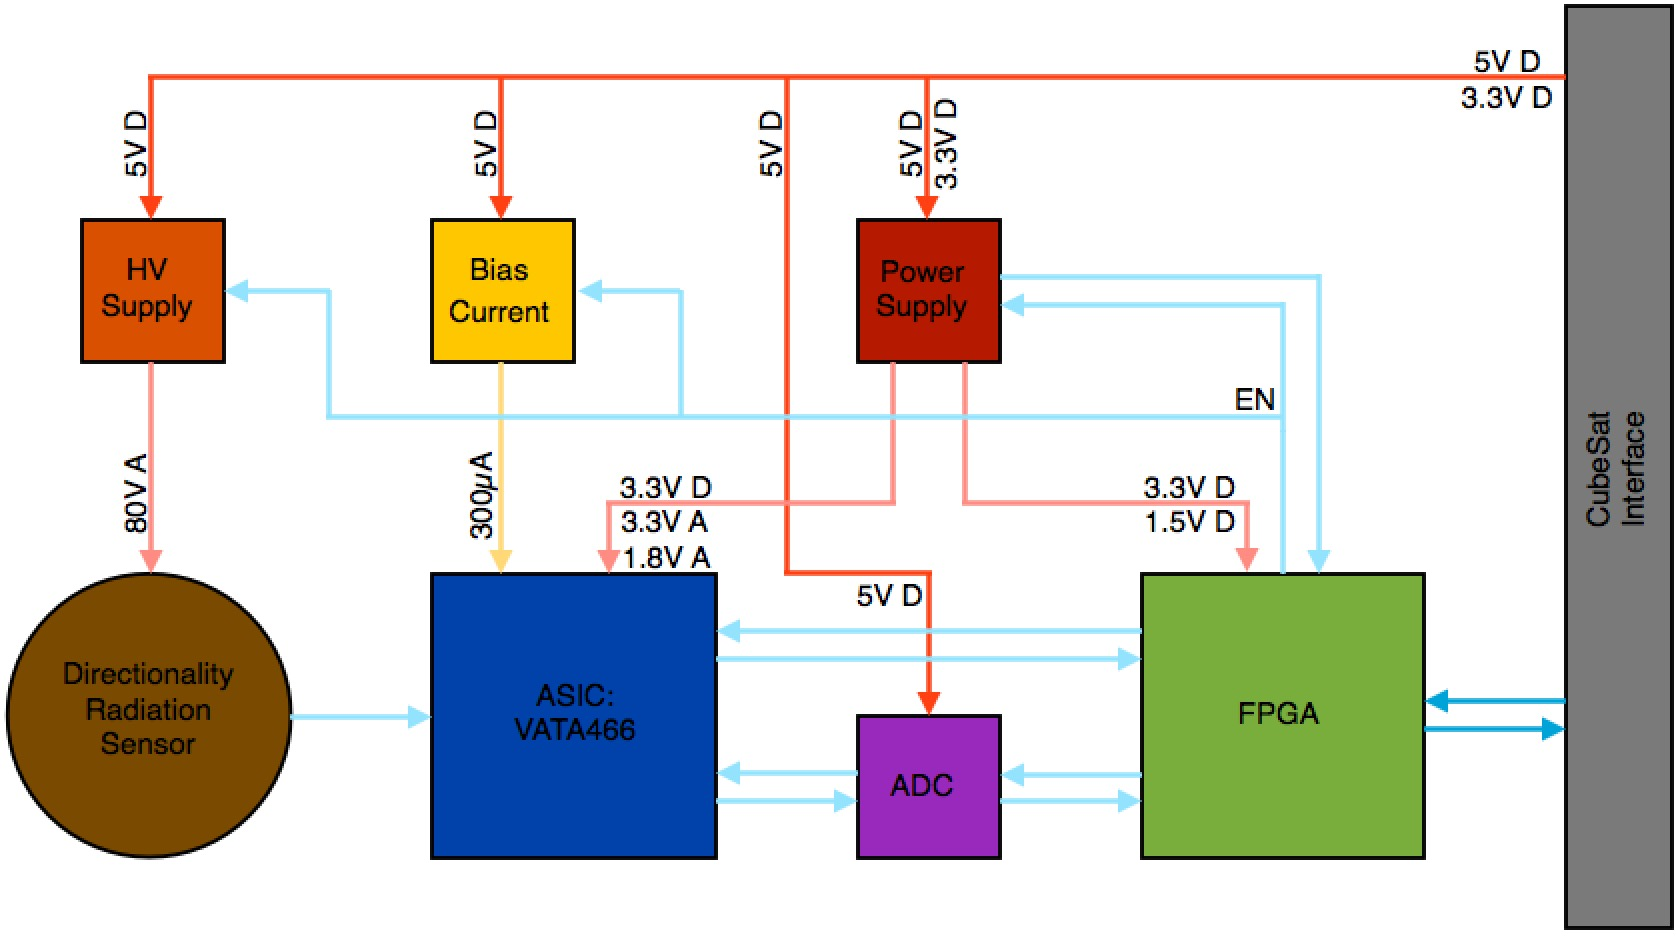
\includegraphics[width=1\textwidth]{electronic_block_diagram.jpg}
    \caption[Block Diagram Readout Electronics]{Block diagram of directional radiation sensor's readout electronics. \\    (Power: Red Arrows; Data: Blue Arrows)}
    \label{fig:electronic_block_diagram}
\end{figure}

The design has to be optimized in terms of power consumption, size and radiation hardness. 
For the latter it was discussed with PSI that the final design could be tested for it's radiation resistance and therefore much cheaper and not officially radiation hardened components can be chosen.
Size and power considerations mainly have to be traded-off against signal quality.
% * <kosheira@gmail.com> 2017-01-13T18:48:56.397Z:
%
% ^.
It is important to stay in the boundaries given by the data sheet of the ASIC to ensure a correct functioning of the instrument.


\subsection{VATA466 Baseboard}
\label{sec:vata466_baseboard}


\subsection{High Voltage Supply}
\label{sec:hv_supply}


\subsection{Directionality Sensor}
\label{sec:directionality Sensor}


\subsection{Supply Voltages}
\label{sec:power_supplies}
- trade-off housekeeping

\subsubsection{Analog Supply Voltages}
\label{sec:analog_supply}
- 1.8 V, 3.3 V
- digital vs opto copplers

\subsection{Bias Current}
\label{sec:bias_current}


\subsection{Analog Digital Converter}
\label{sec:adc}


\subsection{Interface CubeSat}
\label{sec:interface_cubesat}
